\newcommand{\wormTagResultsAucTable}{
    \begin{table}[H]
        \centering
        \begin{tabular}{|p{2,8cm}||P{2,4cm} P{2,4cm} P{2,4cm}|}
            \hline
            Worm Tag & ALOHA\newline (M/B only) & ALOHA & Proposed\newline Model \\
            \hline
            AUC-ROC & - & \textBF{0.975$\pm$0.007} & 0.964$\pm$0.002 \\
            \hline
        \end{tabular}
        \caption[Worm Tag prediction task AUC-ROC results]{AUC-ROC (Area Under Curve) of the different models for the \textbf{Worm Tag} prediction task. Results were aggregated over \textBF{2} training runs with different weight initializations and minibatch orderings. Best results are shown in \textbf{bold}.} \label{tab:wormTag_auc}
    \end{table}
}

\newcommand{\wormTagResultsAtFprTable}{
    \begin{center}
        \begin{longtable}[c]{|P{3,2cm}||P{1,8cm} P{1,8cm} P{1,8cm} P{1,8cm} P{1,8cm}|}
            \hline
            Worm Tag & \multicolumn{5}{c|}{{FPR}} \\
            & $10^{-5}$ & $10^{-4}$ & $10^{-3}$ & $10^{-2}$ & $10^{-1}$ \\
            \hline
            \endfirsthead

            \caption*{\raggedright ...continued from previous page} \\
            \hline
            Worm Tag & \multicolumn{5}{c|}{\textbf{FPR}} \\
            & $10^{-5}$ & $10^{-4}$ & $10^{-3}$ & $10^{-2}$ & $10^{-1}$ \\
            \hline
            \endhead

            \caption*{\raggedleft ...continued on next page} \\
            \endfoot

            \caption[Worm Tag prediction task results]{Mean and standard deviation results (TPR, Accuracy, Recall, Precision and F1-Score) of the different models for the \textbf{Worm Tag} prediction task at different \textbf{FPR}s (\textit{False Positive Rates}). Results were aggregated over \textBF{2} training runs with different weight initializations and minibatch orderings. Best results are shown in \textbf{bold}. Under \textbf{TPR} results are also presented the percentage reduction in mean detection error and in ROC curve standard deviation introduced by the \textit{Proposed Model} with respect to both \textit{ALOHA} model and \textit{Joint Embedding}.} \label{tab:wormTag_results_at_fpr} \\
            \endlastfoot

            \multicolumn{6}{|c|}{\textbf{TPR}} \\
            \hline
            ALOHA (M/B only) & - & - & - & - & - \\
            ALOHA & \textBF{0.221$\pm$0.033} & 0.378$\pm$0.026 & 0.521$\pm$0.068 & 0.611$\pm$0.017 & \textBF{0.925$\pm$0.047} \\
            Proposed Model & 0.179$\pm$0.135 & \textBF{0.398$\pm$0.006} & \textBF{0.608$\pm$0.011} & \textBF{0.669$\pm$0.008} & 0.813$\pm$0.021 \\
            \hline
            Error Reduction wrt\newline ALOHA (M/B only) & - & - & - & - & - \\
            Error Reduction wrt\newline ALOHA & -5.4\% & 3.2\% & 18.2\% & 14.9\% & -149.3\% \\
            \hline
            Std Reduction wrt\newline ALOHA (M/B only) & - & - & - & - & - \\
            Std Reduction wrt\newline ALOHA & -309.1\% & 76.9\% & 83.8\% & 52.9\% & 55.3\% \\
            \hline
            \multicolumn{6}{|c|}{\textbf{Accuracy}} \\
            \hline
            ALOHA (M/B only) & - & - & - & - & - \\
            ALOHA & \textBF{0.877$\pm$0.005} & 0.901$\pm$0.004 & 0.923$\pm$0.011 & 0.930$\pm$0.003 & \textBF{0.904$\pm$0.007} \\
            Proposed Model & 0.870$\pm$0.021 & \textBF{0.905$\pm$0.001} & \textBF{0.937$\pm$0.002} & \textBF{0.939$\pm$0.001} & 0.886$\pm$0.003 \\
            \hline
            \multicolumn{6}{|c|}{\textbf{Recall}} \\
            \hline
            ALOHA (M/B only) & - & - & - & - & - \\
            ALOHA & \textBF{0.221$\pm$0.033} & 0.378$\pm$0.026 & 0.521$\pm$0.068 & 0.611$\pm$0.017 & \textBF{0.925$\pm$0.047} \\
            Proposed Model & 0.179$\pm$0.135 & \textBF{0.398$\pm$0.006} & \textBF{0.608$\pm$0.011} & \textBF{0.669$\pm$0.008} & 0.813$\pm$0.021 \\
            \hline
            \multicolumn{6}{|c|}{\textbf{Precision}} \\
            \hline
            ALOHA (M/B only) & - & - & - & - & - \\
            ALOHA & \textBF{1.000$\pm$0.000} & \textBF{0.999$\pm$0.000} & 0.990$\pm$0.001 & 0.920$\pm$0.002 & \textBF{0.635$\pm$0.012} \\
            Proposed Model & 0.999$\pm$0.001 & \textBF{0.999$\pm$0.000} & \textBF{0.991$\pm$0.000} & \textBF{0.926$\pm$0.001} & 0.605$\pm$0.006 \\
            \hline
            \multicolumn{6}{|c|}{\textbf{F1 Score}} \\
            \hline
            ALOHA (M/B only) & - & - & - & - & - \\
            ALOHA & \textBF{0.361$\pm$0.044} & 0.547$\pm$0.028 & 0.680$\pm$0.059 & 0.734$\pm$0.013 & \textBF{0.753$\pm$0.024} \\
            Proposed Model & 0.281$\pm$0.197 & \textBF{0.569$\pm$0.006} & \textBF{0.753$\pm$0.009} & \textBF{0.777$\pm$0.006} & 0.694$\pm$0.012 \\
            \hline
        \end{longtable}
    \end{center}
}

\newcommand{\wormTagResultsSummaryTable}{
    \begin{table}[H]
        \centering
        \begin{tabular}{|P{3,2cm}||P{1,8cm} P{1,8cm} P{1,8cm} P{1,8cm} P{1,8cm}|}
            \hline
            \multicolumn{6}{|c|}{Worm Tag (at FPR $=1\%$)} \\
            \hline
            Model & TPR & Accuracy & Precision & Recall & F1 score \\
            \hline
            ALOHA (M/B only) & - & - & - & - & - \\
            ALOHA & 0.611$\pm$0.017 & 0.930$\pm$0.003 & 0.920$\pm$0.002 & 0.611$\pm$0.017 & 0.734$\pm$0.013 \\
            Proposed Model & \textBF{0.669$\pm$0.008} & \textBF{0.939$\pm$0.001} & \textBF{0.926$\pm$0.001} & \textBF{0.669$\pm$0.008} & \textBF{0.777$\pm$0.006} \\
            \hline
        \end{tabular}
        \caption[Summary of Worm Tag prediction task results]{Summary of the mean and standard deviation results of the different models for the \textbf{Worm Tag} prediction task at \textbf{FPR} $=1\%$. Results were aggregated over \textBF{2} training runs with different weight initializations and minibatch orderings. Best results are shown in \textbf{bold}.} \label{tab:wormTag_result_summary}
    \end{table}
}

\newcommand{\wormTagRocAlohaMB}{
    \begin{figure}[H]
        \vspace*{-0.5cm}
        \centering
        \includegraphics[width=0.6\textwidth]{./results/worm_tag_roc_alohaMB.png}
        \vspace*{-0.2cm}
        \caption[Worm Tag prediction task ALOHA (M/B only) ROC curve]{ROC curve and AUC statistics of \textBF{ALOHA (M/B only)} model for the \textbf{Worm Tag}. The line represents the \textit{mean} TPR at a given FPR, while the shaded region represents the \textit{standard deviation}. Statistics were computed over \textBF{2} training runs, each with random parameter initialization.}
        \label{fig:wormTagRocAlohaMB}
    \end{figure}
}

\newcommand{\wormTagRocAloha}{
    \begin{figure}[H]
        \vspace*{-0.5cm}
        \centering
        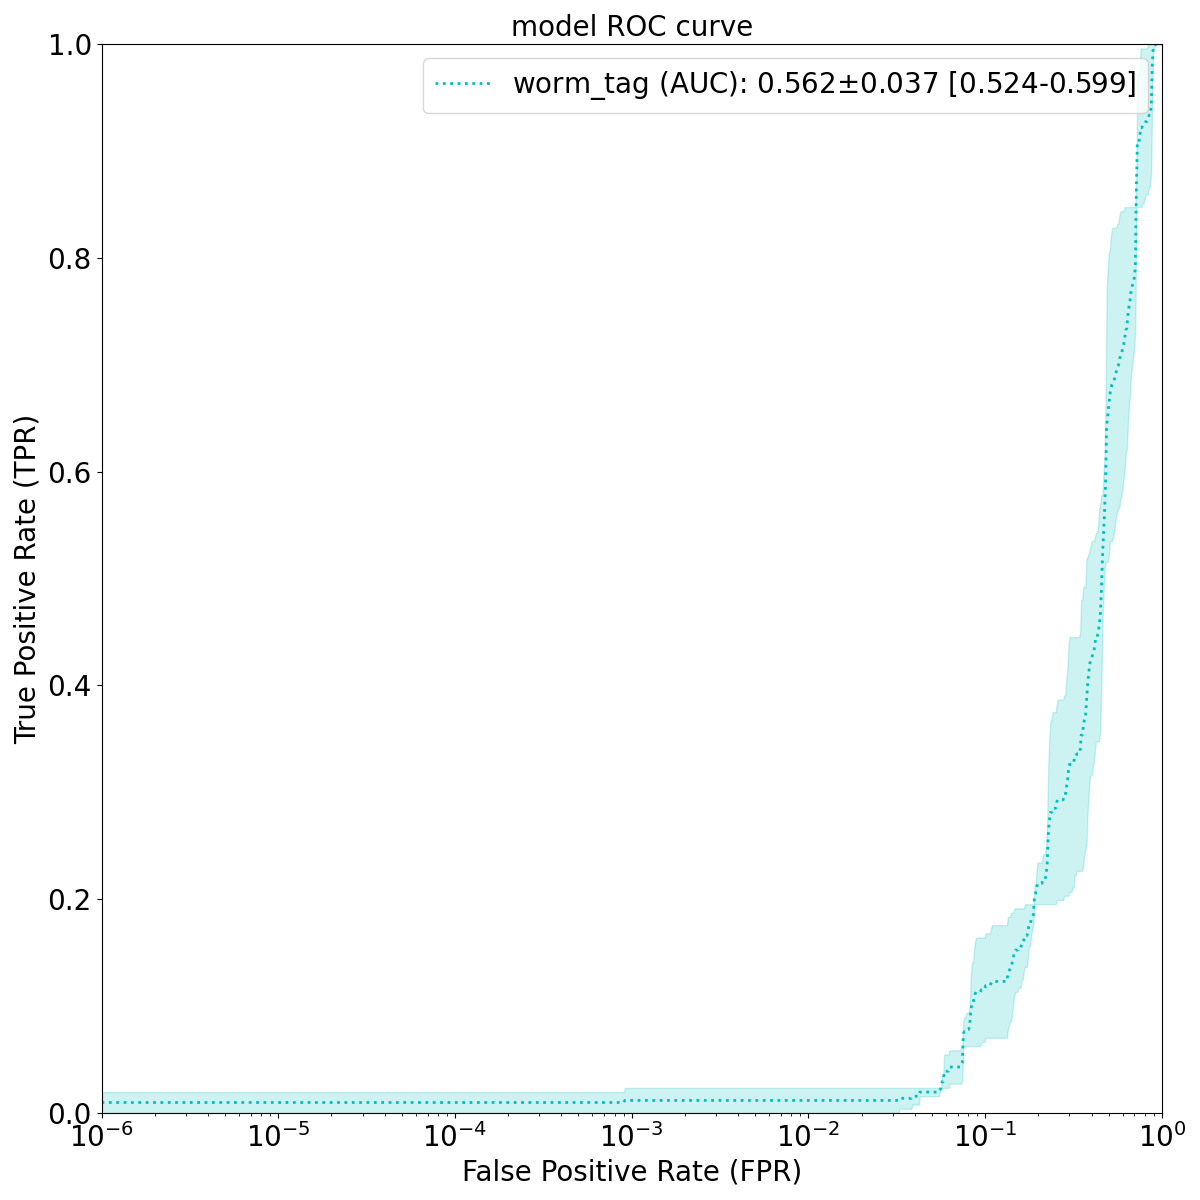
\includegraphics[width=0.6\textwidth]{./results/worm_tag_roc_aloha.png}
        \vspace*{-0.2cm}
        \caption[Worm Tag prediction task ALOHA ROC curve]{ROC curve and AUC statistics of \textBF{ALOHA} model for the \textbf{Worm Tag}. The line represents the \textit{mean} TPR at a given FPR, while the shaded region represents the \textit{standard deviation}. Statistics were computed over \textBF{2} training runs, each with random parameter initialization.}
        \label{fig:wormTagRocAloha}
    \end{figure}
}

\newcommand{\wormTagRocProposedMethod}{
    \begin{figure}[H]
        \vspace*{-0.5cm}
        \centering
        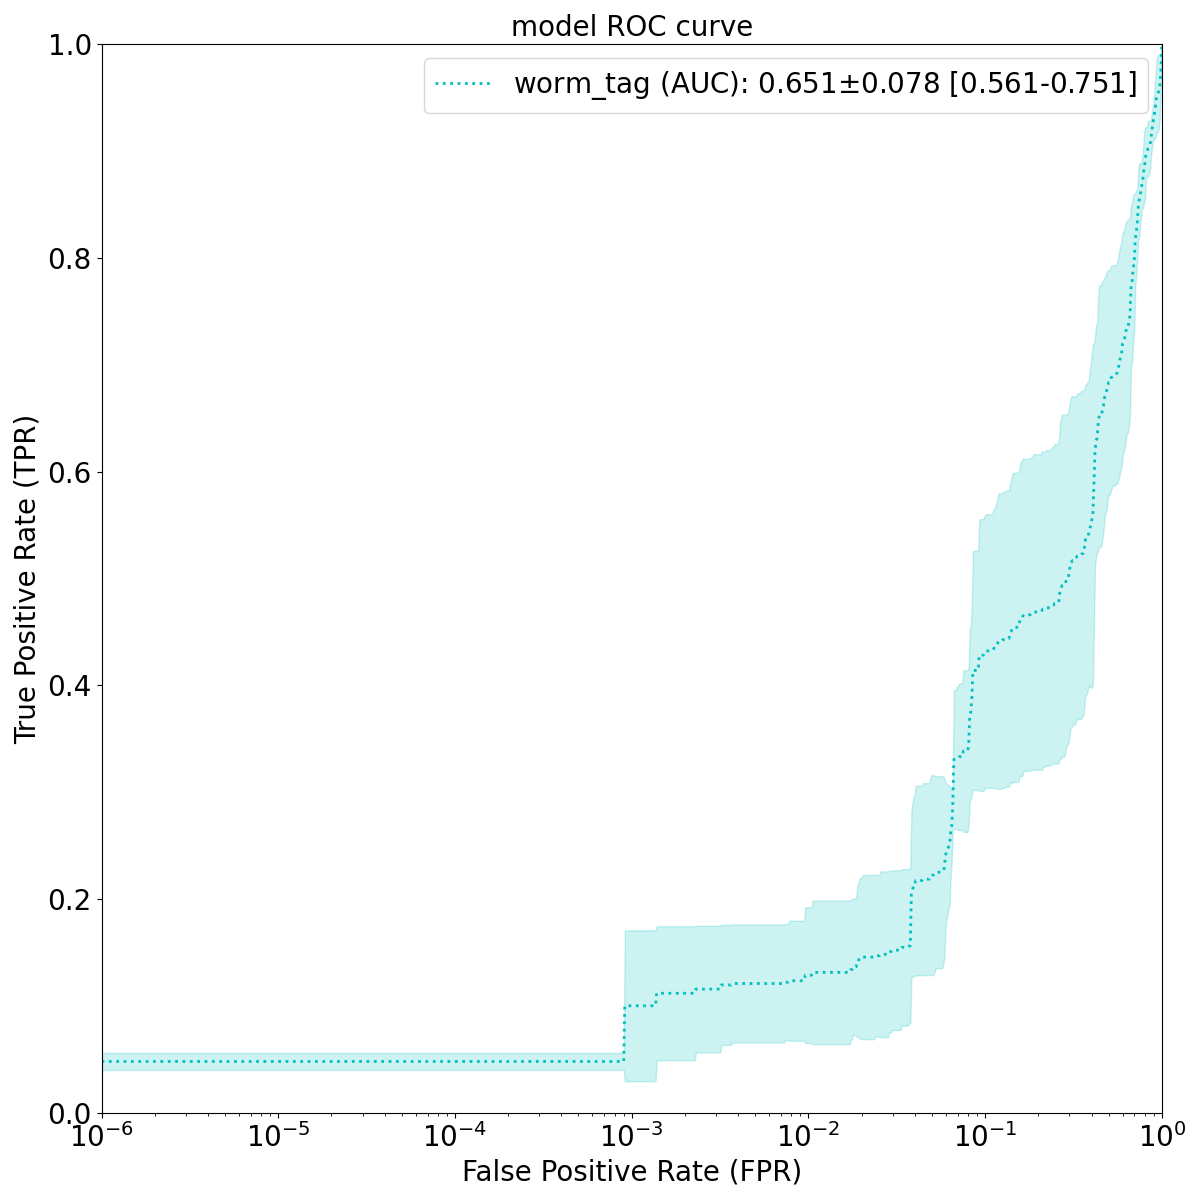
\includegraphics[width=0.6\textwidth]{./results/worm_tag_roc_proposedModel.png}
        \vspace*{-0.2cm}
        \caption[Worm Tag prediction task Proposed Model ROC curve]{ROC curve and AUC statistics of \textBF{Proposed Model} for the \textbf{Worm Tag}. The line represents the \textit{mean} TPR at a given FPR, while the shaded region represents the \textit{standard deviation}. Statistics were computed over \textBF{2} training runs, each with random parameter initialization.}
        \label{fig:wormTagRocProposedModel}
    \end{figure}
}
